\documentclass[thesis.tex]{subfile}

\chapter{Space-tiling and the Devito compilation process}
\label{ch:devito}

We reviewed Devito's motivation and overall architecture in Section~\ref{sec:devito}.
% TODO: elaborate
This chapter examines the details of the existing Devito compilation process pertinent to our implementation of time-tiling, in particular the existing implementation of spatial-tiling (Section~\ref{sec:spatial-tiling}).

In general, we have assumed that Devito only performs valid transformations, which we verify against its extensive test suite.
Therefore, we are only concerned with the transformations that occur between skewing and tiling.


\section{Overview}
Devito generates computations using finite-difference methods to solve differential equations, which are defined using \emph{SymPy}.
These are defined as operators, which define a problem domain and the equations to be applied (Figure~\ref{lst:devito-op}).
A stencil is then derived, optimised, and placed into loops, which are further optimised.

\begin{figure}[!ht]
\begin{lstlisting}[language=Python]
def operator(shape, **kwargs):
    grid = Grid(shape=shape)
    spacing, a, c = 0.1, 0,5, 0,5
    dx2, dy2 = spacing**2, spacing**2
    dt = dx2 * dy2 / (2 * a * (dx2 + dy2))

    # Allocate the grid and set initial condition
    u = TimeFunction(name='u', grid=grid, time_order=2, space_order=2)
    u.data[0, :] = np.linspace(1e-20, 2e-20,
                               num=reduce(mul, shape)).reshape(shape)

    # Derive the stencil according to devito conventions
    eqn = Eq(u.dt, a * (u.dx2 + u.dy2) - c * (u.dxl + u.dyl))
    stencil = solve(eqn, u.forward, rational=False)[0]
    op = Operator(Eq(u.forward, stencil), **kwargs)

    # Execute the generated Devito stencil operator
    op.apply(u=u, t=10, dt=dt)
    return u.data[1, :], op
\end{lstlisting}
	\caption{Defining and applying an operator in Devito. Some set-up is required to define the equation, here a Laplace operator in the \(x,y\) dimensions. In actual usage, the grid (\texttt{u.data[0]}) would be the input domain. The stencil is derived, then applied to the grid.}
	\label{lst:devito-op}
\end{figure}

Our starting point is the stencil that Devito has generated, following its transformation from stencil optimisation in the DSE until the point where loop tiling is applied in the DLE.
We have chosen to restrict the scope of this chapter to these components, which are pertinent to the time-tiling transformation that we implement in Chapter~\ref{ch:implementation}.


\section{The Devito symbolic engine (DSE)}
\label{sec:dse}

The Devito symbolic engine is responsible for stencil optimisation and common sub-expression elimination (CSE).
At this point the indices and loops have not been generated yet, but we have generated the stencil and know its data dependencies.

Although we are working with loop transformations, we will perform skewing (Section~\ref{sec:skewing}) in the DSE, as skewing is a modification to the canonical indexing scheme.

\subsection{Common sub-expression elimination (CSE)}
The purpose of CSE is to reduce redundant computation, by removing duplicate expressions~\cite{muchnick-acdi}.
Figure~\ref{lst:cse-valid} illustrates a situation in which CSE would be used.
In this situation, CSE would remove the two expressions, replacing it with one that subtracted \texttt{0.5F*u[time][x][y][z]}.

\begin{figure}[!ht]
\begin{lstlisting}
float tcse0 = -1.0F*u[time][x][y][z] + ...
              + .5F*u[time][x][y][z];
\end{lstlisting}
	\caption{Code (from Devito) eligible for common sub-expression elimination. Formatting is my own.}
	\label{lst:cse-valid}
\end{figure}

In the DSE, this is also performed at a higher level.
There is a balance to be made here: time-invariant expressions are first separated and assigned to temporaries, avoiding needless CSE, thus decreasing code-generation time.

\subsection{Indexing}
Indexing in Devito is the transformation of a stencil equation with distance co-ordinates to an expression of an indexed data access.
It is a transformation between internal representations of the stencil.

% TODO: consider example

Despite being considered a loop transformation, we have chosen to perform skewing before any indexing occurs, for reasons which will be clear in the next chapter.
However, it is equally valid and perhaps more intuitive to skew after indexing.


\section{The Devito loop engine (DLE)}
\label{sec:dle}

The DLE performs loop transformations including loop fission and tiling, while also marking loops to be executed in parallel or that denormal numbers should be flushed.
Before it is invoked, the loops are built from the previously-manipulated expressions; clearly it would not be possible to implement tiling before this stage.

\subsection{Loop fission}
Loop fission splits a loop to improve data locality.
If the body of a loop nest contains code that can be split into otherwise independent parts, it may be a candidate for loop fission (Figure~\ref{lst:fission-valid}), especially the body can be computed in parallel~\cite{page2009}.
By evaluating the loops one after another, the amount of cache available to each computation increases, resulting in a speedup.

% TODO
\begin{figure}[!ht]
\begin{lstlisting}
for (int x = x_s; x < x_e; x++){
  A[x] = A[x-1] + A[x-2];
  B[x] = B[x-1] + B[x-3];
}
\end{lstlisting}
	\caption{A loop nest on which loop fission would be valid.}
	\label{lst:fission-valid}
\end{figure}

We can easily see that this does not affect space-tiling in Devito, as it has no impact on array indices, since the resultant loops appear in the same nest as the original loop, with the variables duplicated.
Likewise, this holds equally for time-tiling.

\subsection{OpenMP pragmas and parallelisation}
Another particularly relevant operation of the DLE is the addition of OpenMP pragmas indicating that a particular loop may be parallelised~\cite{openmp-spec}.

% TODO: example

While this transformation is performed after tiling, it is pertinent as loops must be marked as parallelisable in the intermediate representation.
Loop tiling generates new loops from old, usually resulting in loop nests that are twice as deep.
It is important to note which of the original loops can be parallelised, and consequently, which of the tiled loops can be parallelised.
This is not a major concern for spatial tiling, as seen in Section~\ref{sec:spatial-tiling}, but will later be important in time-tiling.


\section{Spatial tiling in Devito}
\label{sec:spatial-tiling}

Under the existing tiling transformation in Devito, tiling is performed over every spatial dimension.
Note that the innermost dimension may be vectorised instead.

With spatial tiling, dependencies do not cross tile boundaries, instead only referencing values computed in the previous time iteration.
Therefore, skewing is not required.

\subsection{Remainder loops}
\label{sec:remainder-loops}

When discussing loop tiling in Section~\ref{sec:bg-loop-tiling}, we constrained our tiles with \texttt{min} constraints.
To deal with the case when the tile size does not divide the extent of the iteration space, Devito instead implements \emph{remainder loops}, which Figures~\ref{fig:tiled-remainder-space} and~\ref{lst:remainder} illustrate.

\begin{figure}[!ht]
	\centering
	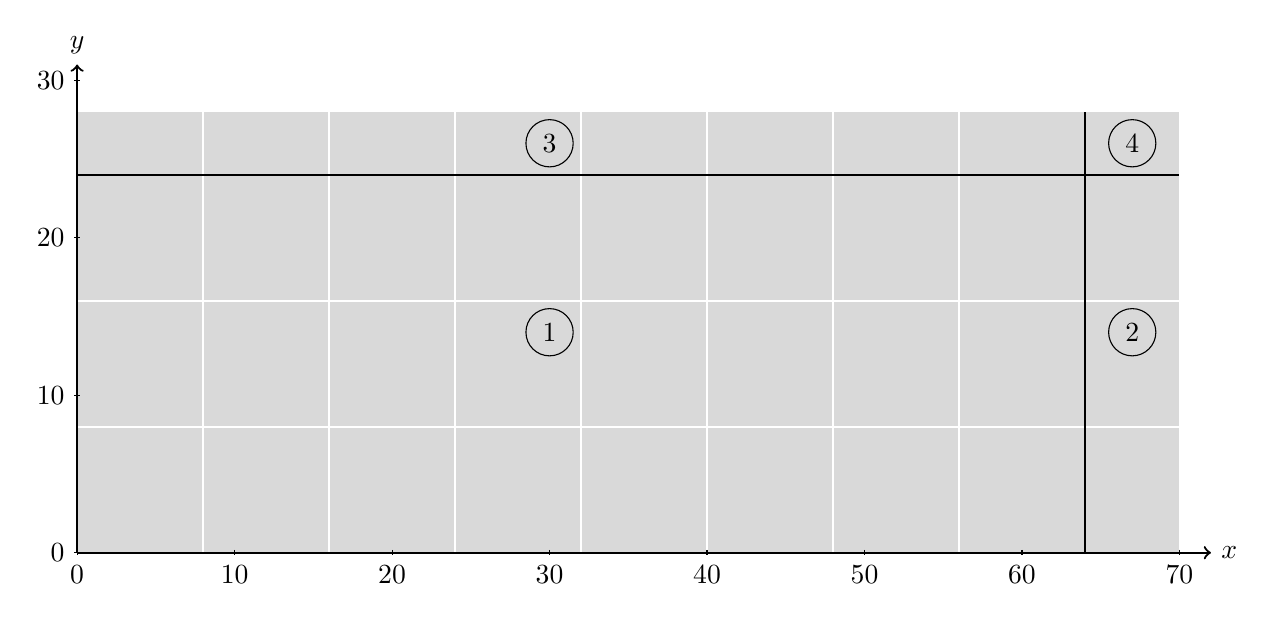
\begin{tikzpicture}
	\fill[gray!30!white] (0,0) rectangle (14,5.6);
	\draw[step=1.6cm,white,thick] (0,0) grid (14,5.6);
	
	\draw[thick,->] (0,0) -- (14.4,0) node[right]{$x$};
	\draw[thick,->] (0,0) -- (0,6.2) node[above]{$y$};
	
	\foreach \x in {0,10,20,30,40,50,60,70}
	\draw (\x*0.2 cm,1pt) -- (\x*0.2 cm,-1pt) node[anchor=north] {$\x$};
	\foreach \y in {0,10,20,30}
	\draw (1pt,\y*0.2 cm) -- (-1pt,\y*0.2 cm) node[anchor=east] {$\y$};
	
	\draw[xstep=12.8,ystep=4.8,black,thick] (0,0) grid (14,5.6);
	\draw (6,2.8) circle [radius=0.3] node {$1$};
	\draw (13.4,2.8) circle [radius=0.3] node {$2$};
	\draw (6,5.2) circle [radius=0.3] node {$3$};
	\draw (13.4,5.2) circle [radius=0.3] node {$4$};
	\end{tikzpicture}
	\caption{Tiles over an iteration space. Note that the tile size need not be the same in each dimension, or divide the extent of the iteration cleanly.}
	\label{fig:tiled-remainder-space}
\end{figure}

\begin{figure}[!ht]
\begin{lstlisting}
for (int x_blk = x_s; x_blk < x_e - (x_e-x_s)%x_bs; x_blk += x_bs)
  for (int y_blk = y_s; y_blk < y_e - (y_e-y_s)%y_bs; y_blk += y_bs)
    for (int x = x_blk; x < x_blk + x_bs; x++)
      for (int y = y_blk; y < y_blk + y_bs; y++)
        A[x][y] = B[x][y] + B[x][y+1];  // Nest 1

for (int x = x_e - (x_e-x_s)%x_bs; x < x_e; x++)
  for (int y_blk = y_s; y_blk < y_e - (y_e-y_s)%y_bs; y_blk += y_bs)
    A[x][y] = B[x][y] + B[x][y+1];  // Nest 2

for (int x_blk = x_s; x_blk < x_e - (x_e-x_s)%x_bs; x_blk += x_bs)
  for (int y = y_e - (y_e-y_s)%y_bs; y < y_e; y++)
    A[x][y] = B[x][y] + B[x][y+1];  // Nest 3

for (int x = x_e - (x_e-x_s)%x_bs; x < x_e; x++)
  for (int y = y_e - (y_e-y_s)%y_bs; y < y_e; y++)
    A[x][y] = B[x][y] + B[x][y+1];  // Nest 4
\end{lstlisting}
	\caption{Replacement of \texttt{min} constraints of Figure~\ref{lst:interchange} with remainder loops. First the main tiles, then the remainder in \texttt{x} then \texttt{y} dimensions, and finally the remainders in both dimensions. Nest numbering according to Figure~\ref{fig:tiled-remainder-space}. Braces removed for concision.}
	\label{lst:remainder}
\end{figure}

\subsection{Determination of tile sizes}
One notes that the loop tiling method includes code to match tile sizes from a user-provided parameter and check their validity.
Nevertheless, this is not relevant to the discussion of time-tiling in this report, apart from the straightforward addition of another dimension.
Therefore, it is omitted from this section.
